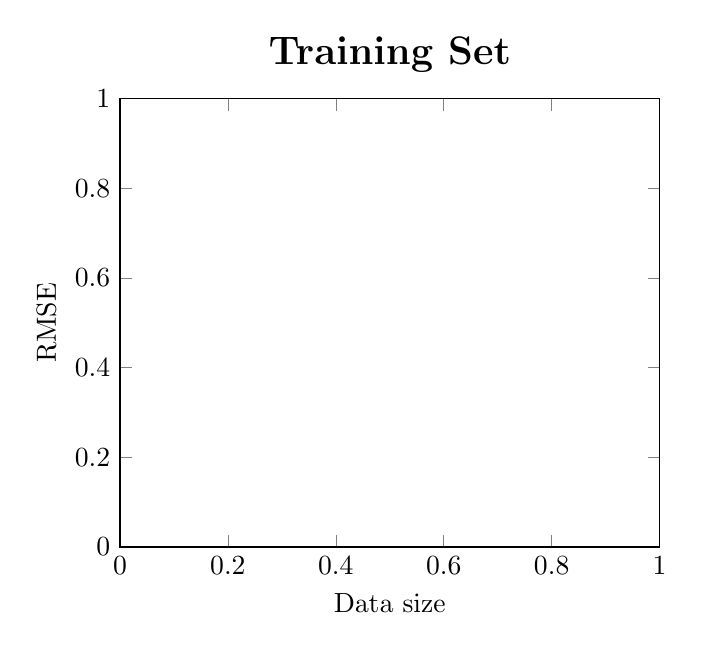
\begin{tikzpicture}
\begin{axis}[
      title = {\bf \Large Training Set},
      clip  = true,
      scaled y ticks=false,
      scaled x ticks=false,
      enlarge y limits = false,
      enlarge x limits = false,
      ylabel style={align=center},
      ylabel = RMSE,ymin= 0,ymax = 14,
      xlabel= Data size,
      legend cell align={left},
      legend style={at={(axis cs:100,5)},anchor=south west, draw = none, fill = none, font=\fontsize{8}{10}\selectfont}, 
]
\errorband{./../output/constant.txt}{0}{1}{2}{cyan}{0.4}	
\addlegendentry{Constant predictor}
\errorband{./../output/linear.txt}{0}{1}{2}{blue}{0.4}	
\addlegendentry{Linear}
\errorband{./../output/kernel.txt}{0}{1}{2}{red}{0.4}	
\addlegendentry{Kernel}
\errorband{./../output/tree.txt}{0}{1}{2}{green}{0.4}	
\addlegendentry{Decision Tree}
\errorband{./../output/forest.txt}{0}{1}{2}{teal}{0.4}	
\addlegendentry{Random forest}
\end{axis}
\end{tikzpicture}

